\documentclass{article}

\usepackage{mystyle}
\setenumerate[0]{label=\alph*.} % Set default of enumerate to be alphabetical
\graphicspath{ {./img/} } % path to image folder


\begin{document}

\maketitle

\newpage

Each part is laid out as follows.

\begin{enumerate}[label=(\roman*)]
\item Hyperparameters
\item Plot of test and train errors through training
\item Output of test and train errors through training
\item Final test and train errors
\item Confusion matrix
\end{enumerate}

I will supply a makefile for loading and running the saved models and output the
train and test errors for each model.

\section{Part 1: MNIST with TensorFlow}

For parts a, b, and c below I used the script \texttt{opt\_hypreparams.py} to find
the optimal hyperparameters, which in this case is the learning rate and the
epoch when we stop training (early stopping to avoid overfitting). For each
model I ran it for the learning rates $(0.1, 0.01, 0.001, 0.0001)$ over 100
epochs with batch size 200, using the
validation set that comes with the mnist dataset in tensorflow I recorded the
validation error at the end of each epoch. For each run I thus got the smallest
validation error, and at what epoch this occurred. From the pairs (learning
rate, optimal epoch) in each run together with the optimal validation error, I
took the pair which yielded the smallest validation error for all runs.
consisting of the following values for each hyperparameter.

There are some weaknesses with this hyperparameter optimization strategy. We are
not optimising over all possible hyperparameters (learning rate, batch size,
epochs), but only over learning rate and epochs. Also, in general random search
is more efficient than grid search. However, for our purposes, I found that this
optimisation gave great results which have to do with that the models here
(1a, 1b, 1c, 1d) have a wide range of hyperparameters which yields good results.

A couple of observations is that all models chose $0.1$ as the optimal learning
rate. This has to do with the fact that TF is numerically stable enough to
handle large learning rates. Since higher learning rates in general means we
converge faster if we do converge, this hints that for learning rate $0.1$ we
converged over the 100 epochs, which maybe didn't happen for the lower learning
rates. This could potentially mean that if we ran the models with a lower
learning rate for a higher number of epochs, we could push the optimal
validation error down further. However, the errors are very good and shows that
each model improves upon the previous ones.
\newpage

\subsection{(a) 1 linear layer, followed by a softmax}

\subsubsection{Optimal hyperparameters}

\begin{description}
\item[learning rate] $0.1$
\item[epochs] $85$
\end{description}

\subsubsection{Graph, confusion matrix and final errors}

The title should be 'Error over iterations'.

\begin{figure}[H]
  \centering
  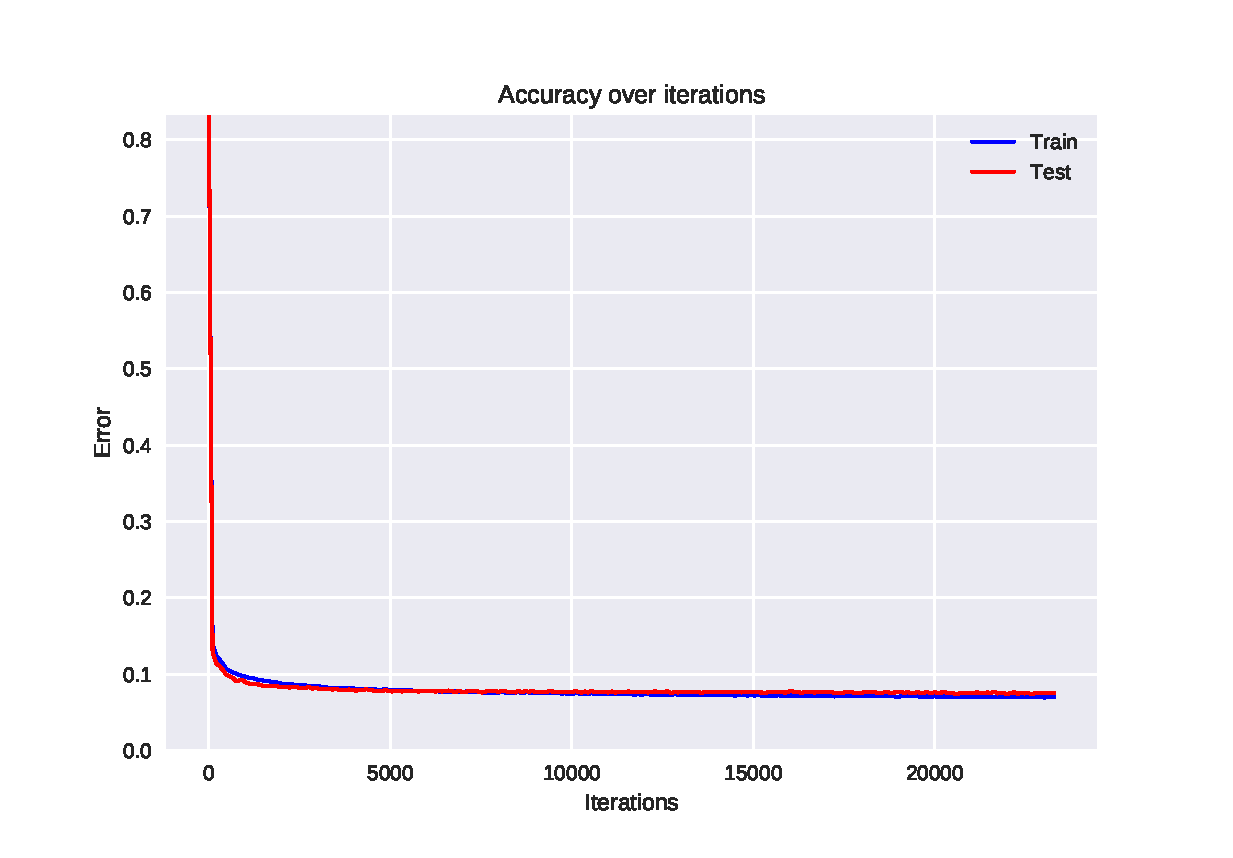
\includegraphics[width=0.95\textwidth]{error_1a.eps}
  \caption{Error plot for model 1a}
  \label{fig:err_1a}
\end{figure}

\begin{figure}[H]
  \centering
  \includegraphics[width=0.95\textwidth]{confusion_matrix_1a.eps}
  \caption{Confusion matrix for model 1a}
  \label{fig:conf_1a}
\end{figure}

Output of training and test error during training of the model

\verbatiminput{./code/Part1/model_1a_output.txt}

\begin{description}
\item[Final train error:] $0.06973$
\item[Final test error:] $0.07620$
\end{description}

\newpage

\subsection{(b) 1 hidden layer (128 units) with a ReLU non-linearity, followed
  by a softmax}

\subsubsection{Optimal hyperparameters}

\begin{description}
\item[learning rate] $0.1$
\item[epochs] $83$
\end{description}

\subsubsection{Graph, confusion matrix and final errors}

The title should be 'Error over iterations'.

\begin{figure}[H]
  \centering
  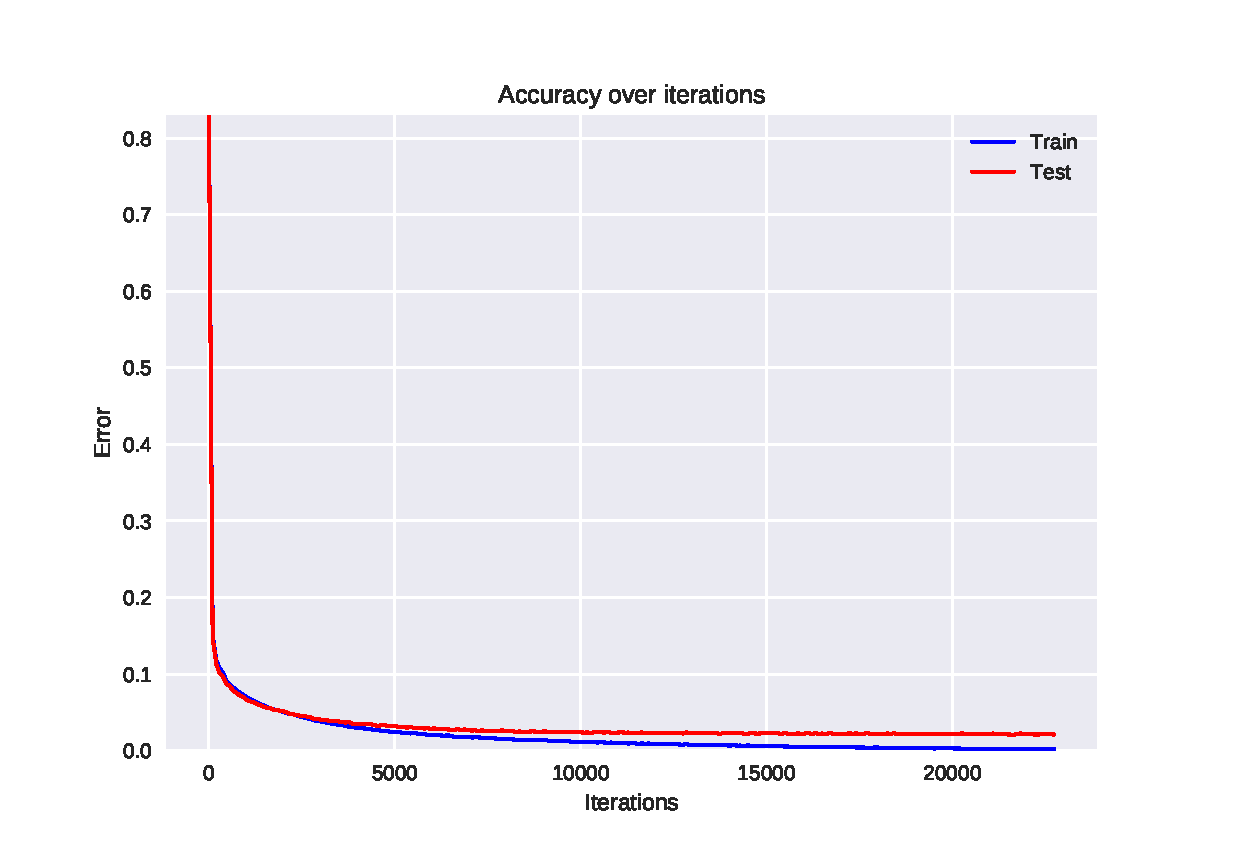
\includegraphics[width=0.95\textwidth]{error_1b.eps}
  \caption{Error plot for model 1b}
  \label{fig:err_1b}
\end{figure}

\begin{figure}[H]
  \centering
  \includegraphics[width=0.95\textwidth]{confusion_matrix_1b.eps}
  \caption{Confusion matrix for model 1b}
  \label{fig:conf_1b}
\end{figure}

Output of training and test error during training of the model

\verbatiminput{./code/Part1/model_1b_output.txt}

\begin{description}
\item[Final train error:] $0.00169$
\item[Final test error:] $0.02140$
\end{description}

\newpage

\subsection{(c) 2 hidden layers (256 units) each, with ReLU non-linearity,
  follow by a softmax}

\subsubsection{Optimal hyperparameters}

\begin{description}
\item[learning rate] $0.1$
\item[epochs] $86$
\end{description}

\subsubsection{Graph, confusion matrix and final errors}

The title should be 'Error over iterations'.

\begin{figure}[H]
  \centering
  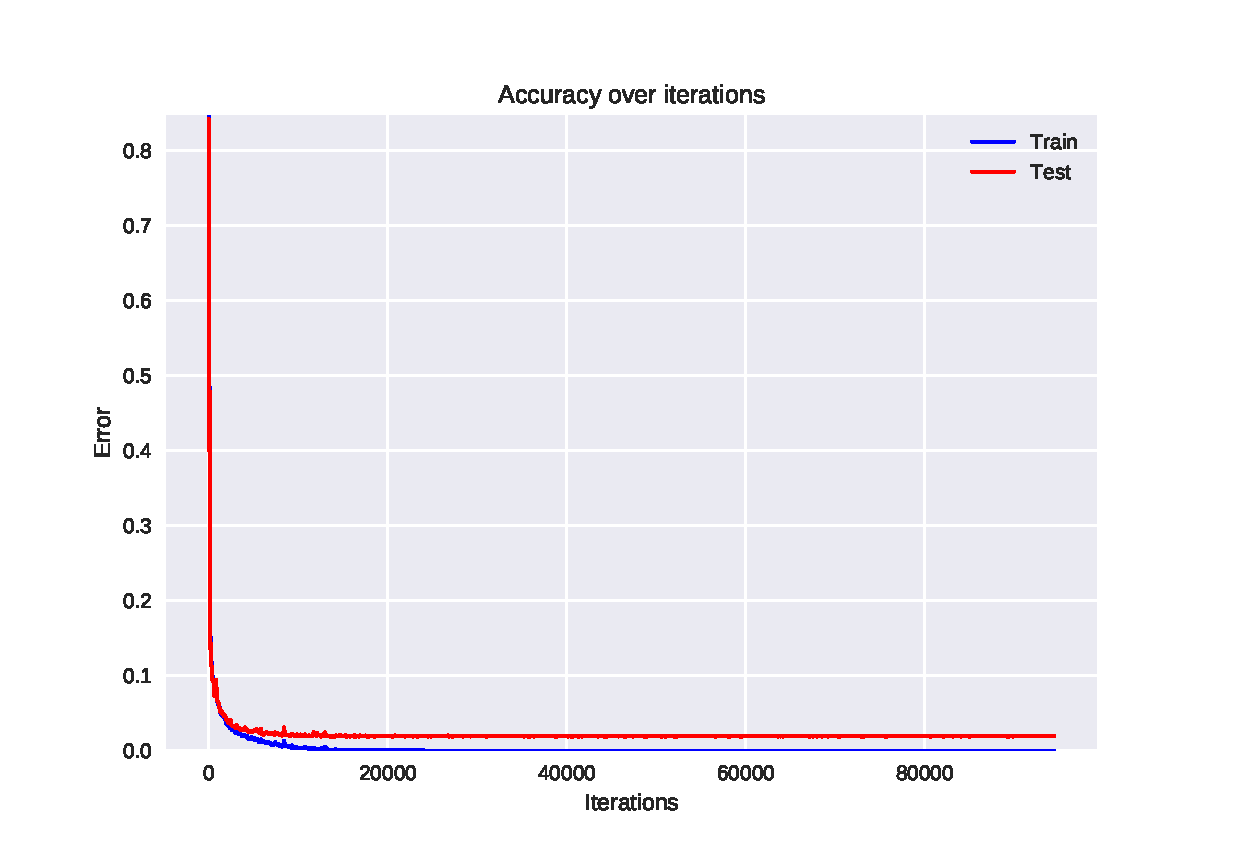
\includegraphics[width=0.95\textwidth]{error_1c.eps}
  \caption{Error plot for model 1c}
  \label{fig:err_1c}
\end{figure}

\begin{figure}[H]
  \centering
  \includegraphics[width=0.95\textwidth]{confusion_matrix_1c.eps}
  \caption{Confusion matrix for model 1c}
  \label{fig:conf_1c}
\end{figure}

Output of training and test error during training of the model

\verbatiminput{./code/Part1/model_1c_output.txt}

\begin{description}
\item[Final train error:] $0.00000$
\item[Final test error:] $0.01890$
\end{description}

\newpage

\subsection{(d) 3 layer convolutional model, followed by a softmax}

\subsubsection{Optimal hyperparameters}

\begin{description}
\item[learning rate] $0.1$
\item[epochs] $53$
\end{description}

\subsubsection{Graph, confusion matrix and final errors}

The title should be 'Error over iterations'.

\begin{figure}[H]
  \centering
  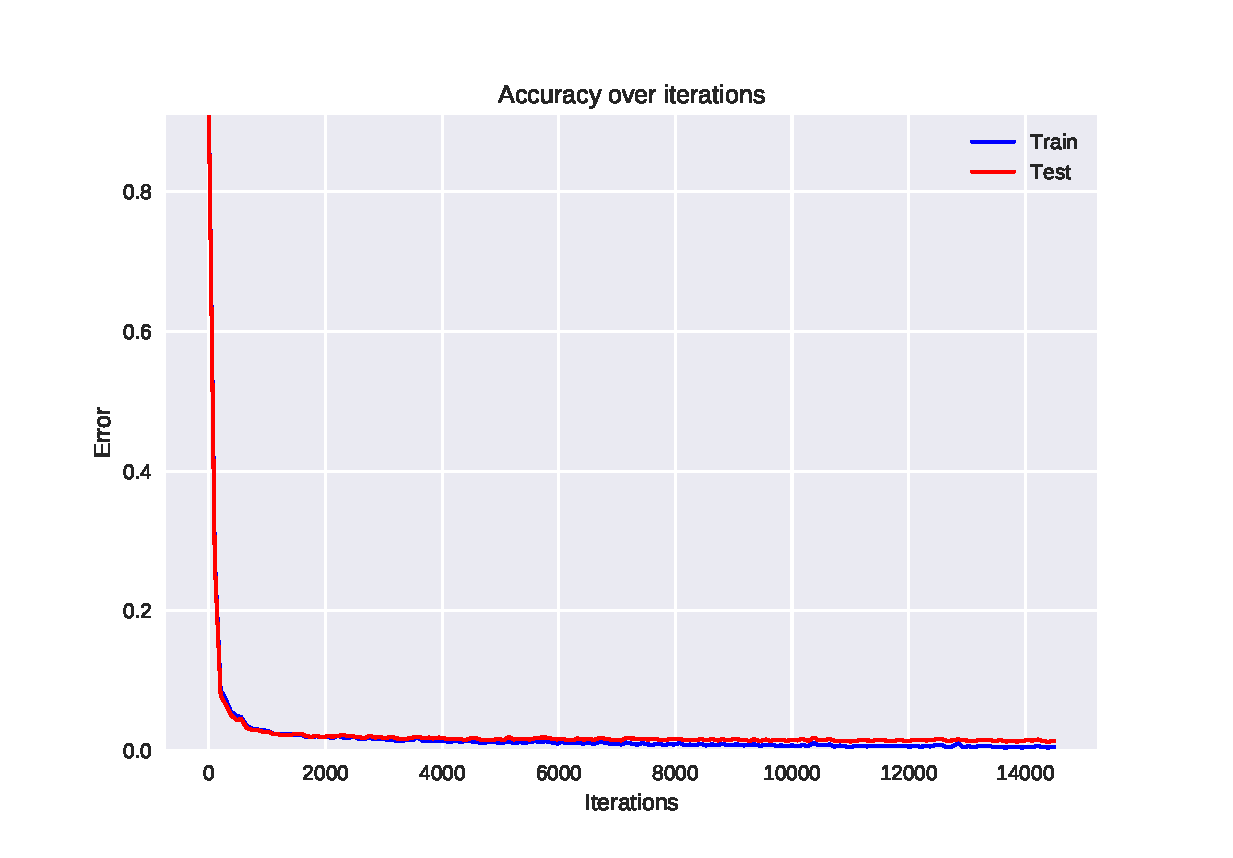
\includegraphics[width=0.95\textwidth]{error_1d.eps}
  \caption{Error plot for model 1d}
  \label{fig:err_1d}
\end{figure}

\begin{figure}[H]
  \centering
  \includegraphics[width=0.95\textwidth]{confusion_matrix_1d.eps}
  \caption{Confusion matrix for model 1d}
  \label{fig:conf_1d}
\end{figure}

\verbatiminput{./code/Part1/model_1d_output.txt}

\begin{description}
\item[Final train error:] $0.00707$
\item[Final test error:] $0.01400$
\end{description}

\newpage

\section{Part 2: MNIST without TensorFlow}

Note: I have by convention put the models of TF and numpy (implementation) in a
correspondence such that throughout the document I call the first model model a,
the second model model b and so on. This also means that my code follows this
convention. This also means that I name the models 1a,
1b, 1c and 1d and for part 2 I name them model 2a, 2b, 2c, 2d, where the models
(1a, 2a), (1b, 2b), (1c, 2c), (1d, 2d) are the same in terms of architecture.

Consequentially, we instead have Problems like P2:b which corresponds to
implementing model 2a and similarly for P2:c, P2:d and P2:e.

\subsection{(a) Compute the folowing derivatives}

We first introduce some notation. We let $\{x_i, y_i\}$ be the data set with
$y_i$ being the digit and let $t_i$ be the one-shot vector of example $i$.
For an arbitrary module we let $x$ be the input, $z$ be the linear
transformation $z = Wx + b$ and $y = \sigma(z)$, the non-linear mapping. For the
final module we let $p$ be the predicted probability vector over digits. In the
examples below we drop the index on $i$ and just write them as $x, z, y, t, p$.

We have that 

\begin{equation*}
  loss = \sum_{i=1}^N -\log (p(y_i | x_i)) = \sum_{i=1}^N L_i
\end{equation*}

Since derivatives are linear operators, we only care about the derivative of
$L_i$ since if we know that, we know the derivative of the $loss$. We write
$L_i$ as $L$ as we drop the dependency on the example for the time being.

In order to stay consistent with vector notation, we index the classes from $1$
to $10$ meaning that $0$ is in the first class, $1$ in the second and so on. We
can shift this back easily if we want to.

\begin{enumerate}[label=(\roman*)]
\item Derivative of the loss function wrt. the scores $z$: $\pdv{L}{z}$.
  
  We first calculate the element-wise partial derivative of the loss with regards
  to the entry $z_j$, the $j$'th entry of the output logits in the final layer
  of the input $x$. Then
  
  \begin{align*}
    \pdv{L}{z_j} & = \pdv{\log(\sum_{c=1}^{10} \exp(z_{c}))}{z_j} - \pdv{z_{y}}{z_j} \\
                        & = \frac{\exp( z_j ) }{ \sum_{c=1}^{10} \exp(z_{c}) }  - \delta(j = y)
  \end{align*}

  Vectorizing this we have that the gradients can be written as

  \begin{equation*}
    \pdv{L}{z} = (p - t)^T
  \end{equation*}

  where $p$ is the predicted class probabilities given the input $x$ and $t$ is
  the one-hot vector of the true label.

\item Given the model in (P1:a), compute the derivative of the loss wrt input $x$,
  derivative of the loss with to the layer’s parameters $W$ , $b$.

  We have the following explicit relationships from the modules.
  
  \begin{align*}
    z & = Wx + b \implies \\
    z_i & = \sum_{j=1}^n W_{ij} x_j + b_i \\
    p & =  \exp(z) / sum(\exp(z)) \implies \\
    p_i & = \frac{\exp(z_{i})}{\sum_{c=1}^{10} \exp(z_{c})} \\
  \end{align*}

  \begin{enumerate}
  \item

    \begin{align*}
      \pdv{L}{x_i} & = \pdv{L(z_1(x_i), \dots, z_{10}(x_i)}{x_i} \\
                   & = \sum_{c=1}^{10} \pdv{L}{z_{c}} \cdot \pdv{z_c}{x_i} \\
                   & = \sum_{c=1}^{10}(p_c - \delta(y = c)) \sum_{j=1}^{784} ( W_{cj} \pdv{x_j}{x_i} + \pdv{b_c}{x_i} ) \\
                   & = \sum_{c=1}^{10}(p_c - \delta(y = c))W_{ci} \\
                   & = [(p - t)^TW]_i
    \end{align*}

    Hence we can vectorize this as

    \begin{equation*}
      \pdv{L}{x} = (p - t)^TW
    \end{equation*}

  \item

    \begin{align*}
      \pdv{L}{W_{ij}} & = \pdv{L(z_1(W_{ij}), \dots, z_{10}(W_{ij}))}{W_{ij}} \\
                      & = \sum_{c=1}^{10}\pdv{L}{z_c} \cdot \pdv{z_c}{W_{ij}} \\
                      & = \sum_{c=1}^{10}(p_c - \delta(y = c)) \sum_{l=1}^{784} ( \pdv{W_{cl}}{W_{ij}}x_l + \pdv{b_c}{W_{ij}} ) \\
                      & = \sum_{c=1}^{10}(p_c - \delta(y = c))x_j\delta(c = i, l = j) \\
                      & = (p_i - \delta(y = i))x_j
    \end{align*}

    We can write this matrix as

    \begin{equation*}
      \pdv{L}{W}^T =
      \begin{bmatrix}
        (p_1 - \delta(y = 1))x_1 & (p_1 - \delta(y = 1))x_2 & \dots & (p_1 - \delta(y = 1))x_{784} \\
        (p_2 - \delta(y = 2))x_1 & \ddots & & \vdots \\
        \vdots & & & \vdots \\
        (p_{10} - \delta(y = 10))x_1 & \dots & \dots & (p_{10} - \delta(y = ))x_{784} \\
      \end{bmatrix}
    \end{equation*}

    We recognise that this is just an outer product such that we can write

    \begin{equation*}
      \pdv{L}{W} = x(p - t)^T
    \end{equation*}

  \item

    \begin{align*}
      \pdv{L}{b_i} & = \pdv{L(z_1(b_i), \dots, z_{10}(b_i))}{b_i} \\
                   & = \sum_{c=1}^{10}(p_c - \delta(y = c))\sum_{l=1}^{784} ( \pdv{W_{cl}x_l}{b_i} + \pdv{b_c}{b_i}) \\
                   & = \sum_{c=1}^{10}(p_c - \delta(y = c))\delta(c = i)\\
                   & = (p_i - \delta(y = i))
    \end{align*}

    This is the same as for $\pdv{L}{z}$ so we may vectorize this as

    \begin{equation*}
      \pdv{L}{b} = (p - t)^T
    \end{equation*}
    
  \end{enumerate}
  
\item Compute the derivative of a convolution layer wrt. to its parameters $W$ and
  wrt. to its input (4-dim tensor).

  We introduce some notation: We let the input to a 3x3x16 conv2d layer be
  denoted by $I$, where $I$ is a tensor of dimensions $(E, N, N, D)$, where the
  quadruplet by convention represent for all tensors $(example, height, width, depth)$ where
  we start counting from the upper left front corner for the input of each
  example. We let an element of this
  input be indexed by $I(e, x, y, d)$. Similarly we let the output of this layer be
  denoted by $C$, where $C$ is a tensor of dimensions $(E, N, N, Z)$ where the
  width and height of $C$ and $I$ are equal, but the depths are independent of
  each other.

  For this 3x3x16 conv2d layer we let the weight which maps $I(\cdot, \cdot, \cdot,
  \cdot)$ to $C(\cdot, \cdot,
  \cdot, z)$ be denoted by $W^{z}$, where $W^{z}$ is a tensor of dimension $(3,
  3, D)$, and there will be 16 of these weights, $\{W^{1}, \dots, W^{16}\}$, one
  for each output filter.

  For convolution, we let $K = I * W$ denote the image $I$ convoluted with the
  kernel $W$. Specifically in our case, we have that the convolution $K(x, y) =
  \sum_{a, b \in \{-1, 0, 1\}} I(x - a, y - b)W(a, b)$ with padding such that
  $K$ is of the same dimension of $I$, i.e. we let \\$W(\cdot, 0) = W(\cdot, N +
  1) = W(0, \cdot) = W(N + 1, \cdot) = 0$. 

  For our case when the number of channels are greater than one, we have that
  the output can be written as

  \begin{align*}
    C(e, x, y, z) = \sum_{d = 1}^D (I(e, \cdot, \cdot, d) * W^{z}(\cdot, \cdot, d))(x, y) + b^{z}
  \end{align*}

  \begin{enumerate}
  \item Since the only non-trivial case is for when the example is the same for
    both input and output, we drop the dependency on $e$ and assume it to be the
    same for $I$ and $C$

    \begin{align*}
      \pdv{C(i, j, k)}{I(x, y, z)} & = \pdv{\sum_{d = 1}^D (I(\cdot, \cdot, d) * W^{k}(\cdot, \cdot, d))(i, j) + b^{k}}{I(x, y, z)} \\
                                   & = \sum_{d = 1}^D \pdv{(I(\cdot, \cdot, d) * W^{k}(\cdot, \cdot, d))(i, j) + b^{k}}{I(x, y, z)} \\
                                   & = \pdv{(I(\cdot, \cdot, z) * W^{k}(\cdot, \cdot, z))(i, j) + b^{k}}{I(x, y, z)} \\
                                   & = \pdv{(I(\cdot, \cdot, z) * W^{k}(\cdot, \cdot, z))(i, j)}{I(x, y, z)} \\
                                   & = \sum_{a, b \in \{-1, 0, 1\}}  \pdv{I(i - a, j - b, z)}{I(x, y, z)} W^k(a, b, z) \\
    \end{align*}

    From here we see that only the points within one square from $I(x, y, z)$
    (including the diagonals) in the $x-y$-plane and on depth of $z$ will have
    non-zero derivative with respect to $I(x, y, z)$. Assume we have such a
    point, otherwise the expression will be zero, then let $a_{x, i}, b_{y, j}$
    be the indices in $\{-1, 0, 1\}$ such that $(i - a_{x, i}, j - b_{y, j}) =
    (x, y)$. Then we have the final expression

    \begin{align*}
      \pdv{C(i, j, k)}{I(x, y, z)} = W^k(a_{x, i}, b_{y, j}, z)
    \end{align*}

    which in terms of the batch we can write as

    \begin{align*}
      \pdv{C(e_1, i, j, k)}{I(e_2, x, y, z)} = \delta(e_1 = e_2)W^k(a_{x, i}, b_{y, j}, z)
    \end{align*}

  \item Similarly here we drop the dependency since we can just stack the
    examples in a 4d tensor after working it out example by example.

    \begin{align*}
      \pdv{C(i, j, k)}{W^l(x, y, z)} & = \pdv{\sum_{d = 1}^D (I(\cdot, \cdot, d) * W^{k}(\cdot, \cdot, d))(i, j) + b^{k}}{W^l(x, y, z)} \\
                                     & = \sum_{d = 1}^D \pdv{(I(\cdot, \cdot, d) * W^{k}(\cdot, \cdot, d))(i, j) + b^{k}}{W^l(x, y, z)} \\
                                     & = \pdv{(I(\cdot, \cdot, z) * W^{k}(\cdot, \cdot, z))(i, j) + b^{k}}{W^l(x, y, z)} \\
                                     & = \pdv{(I(\cdot, \cdot, z) * W^{k}(\cdot, \cdot, z))(i, j)}{W^l(x, y, z)} \\
                                     & = \sum_{a, b \in \{-1, 0, 1\}} I(i - a, j - b, z)\pdv{W^k(a, b, z)}{W^l(x, y, z)} \\
                                     & = \sum_{a, b \in \{-1, 0, 1\}} I(i - a, j - b, z)\delta(k = l, a = x, b = z) \\
                                     & = I(i - x, j - y, z)\delta(l = k)
    \end{align*}
        
  \end{enumerate}
  
\end{enumerate}

For the part 2 of the network building I have used a modular approach. Using OOP
I let the layers be classes with specific methods that calculate the
backpropagation step and feedforward step, together with helper methods for
setting the input and output of each layer as needed in the backpropagation.

On top of this I built a NeuralNetwork class which takes as input a list of
instances of the layers which then does the training, plotting and various other
methods as needed to get the necessary plots, figures and hyperparameter
optimisation of the models.

For each model I do 3 runs over the learning rate. The learning rate for each
model is picked from the list [$lr_0*10^{-i}$] where $i \in \{0, 1, 2\}$ and
$lr_0$ is the biggest power of ten such that I can train the model without
numerical issues (NaN's and infinities). This meant that for the models (2a, 2b, 2c,
corresponding to the models in part 1) I had initial learning rates ($lr_0$) of
0.1, 0.001 and 0.0001. I run the models (2a, 2b, 2c,
corresponding to the models in part 1) for 150, 300 and 500 epochs each due to
make sure that they converged with respect to the initial learning rates for
each model.
For each finished epoch I record the validation error and add this to a list.
When the run is finished I record the smallest error in this list and at the end
of what epoch this occurred. After each finished run I compare the best error
for this run with the optimal error for any run and set the optimal error to be
the error of this run if it is smaller. In the end I return the learning rate
and the epoch at which the lowest error occurred and set this to the be the
learning rate and the epoch to stop of the model.

I wasn't able to get the CNN to work properly and had to leave it out.

\subsection{(b) Implement and train the model in (P1:a)}

\subsubsection{Optimal hyperparameters}

\begin{description}
\item[epochs] $107$
\item[learning rate] $0.001$
\end{description}

\subsubsection{Graph, confusion matrix and final errors}

The title should be 'Error over iterations'.

\begin{figure}[H]
  \centering
  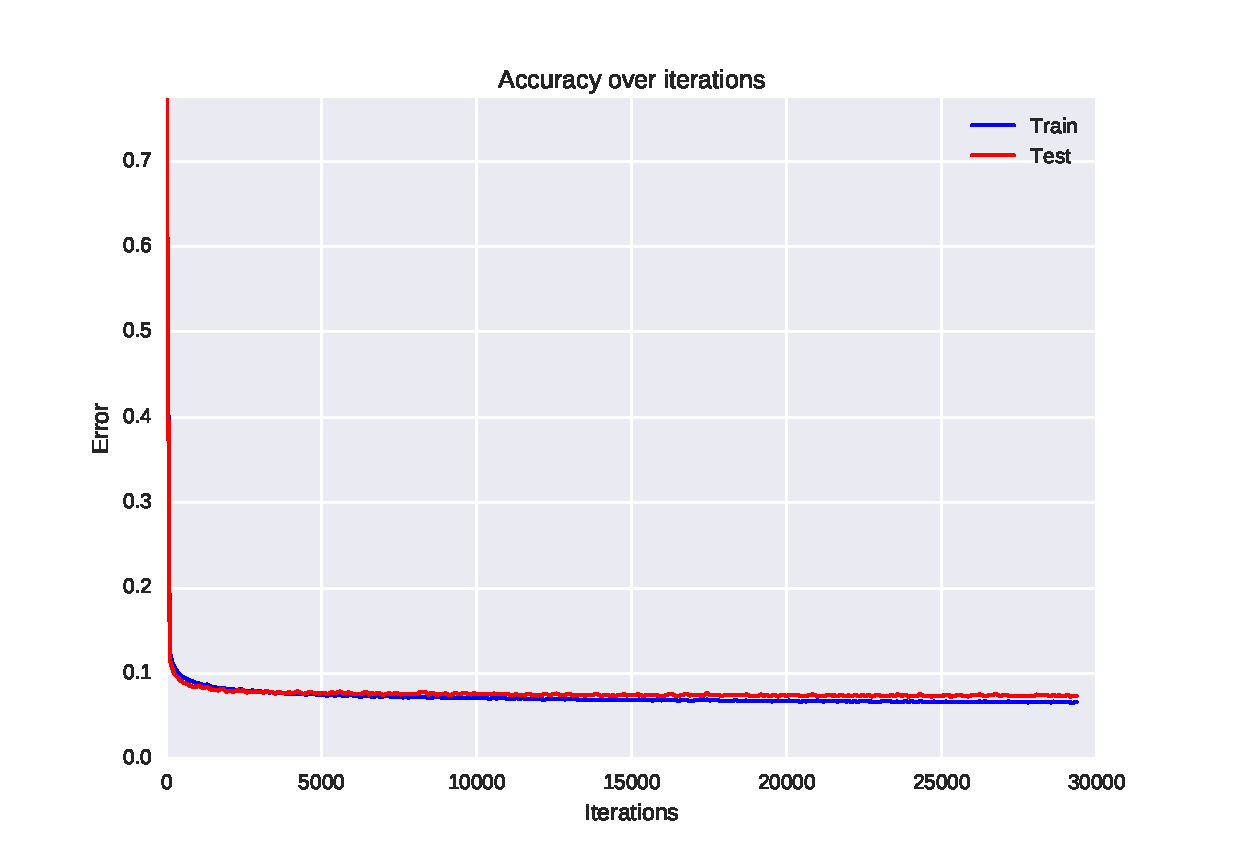
\includegraphics[width=0.95\textwidth]{error_model_2a.eps}
  \caption{Error plot for model 2a}
  \label{fig:err_2a}
\end{figure}

\begin{figure}[H]
  \centering
  \includegraphics[width=0.95\textwidth]{model_2a_confusion_matrix.eps}
  \caption{Confusion matrix for model 2a}
  \label{fig:conf_2a}
\end{figure}

Output of training and test error during training of the model. Due to the large
number of epochs we only show output of every ten epoch and the final epoch.

\verbatiminput{./code/Part2/model_2a_output.txt}

\begin{description}
\item[Final train error:] $0.06604$
\item[Final test error:] $0.07300$
\end{description}

\newpage

\subsection{(c) Implement and train the model in (P1:b)}

\subsubsection{Optimal hyperparameters}

\begin{description}
\item[epochs] $281$
\item[learning rate] $0.0001$
\end{description}

\subsubsection{Graph, confusion matrix and final errors}

The title should be 'Error over iterations'.

\begin{figure}[H]
  \centering
  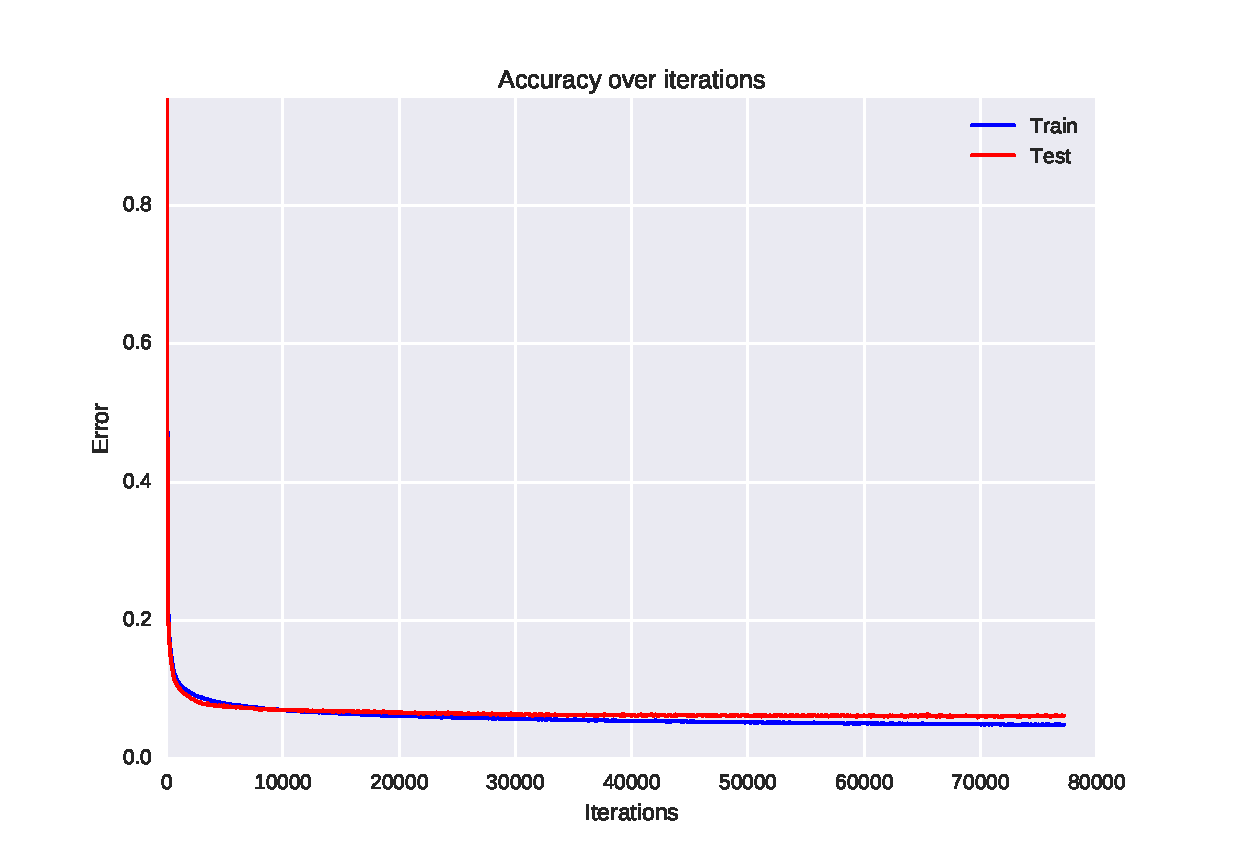
\includegraphics[width=0.95\textwidth]{error_model_2b.eps}
  \caption{Error plot for model 2b}
  \label{fig:err_2b}
\end{figure}

\begin{figure}[H]
  \centering
  \includegraphics[width=0.95\textwidth]{model_2b_confusion_matrix.eps}
  \caption{Confusion matrix for model 2b}
  \label{fig:conf_2b}
\end{figure}

Output of training and test error during training of the model. Due to the large
number of epochs we only show output of every ten epoch and the final epoch.

\verbatiminput{./code/Part2/model_2b_output.txt}

\begin{description}
\item[Final train error:] $0.04887$
\item[Final test error:] $0.06150$
\end{description}

\newpage

\subsection{(d) Implement and train the model in (P1:c)}

\subsubsection{Optimal hyperparameters}

\begin{description}
\item[epochs] $175$
\item[learning rate] $0.0001$
\end{description}

\subsubsection{Graph, confusion matrix and final errors}

The title should be 'Error over iterations'.

\begin{figure}[H]
  \centering
  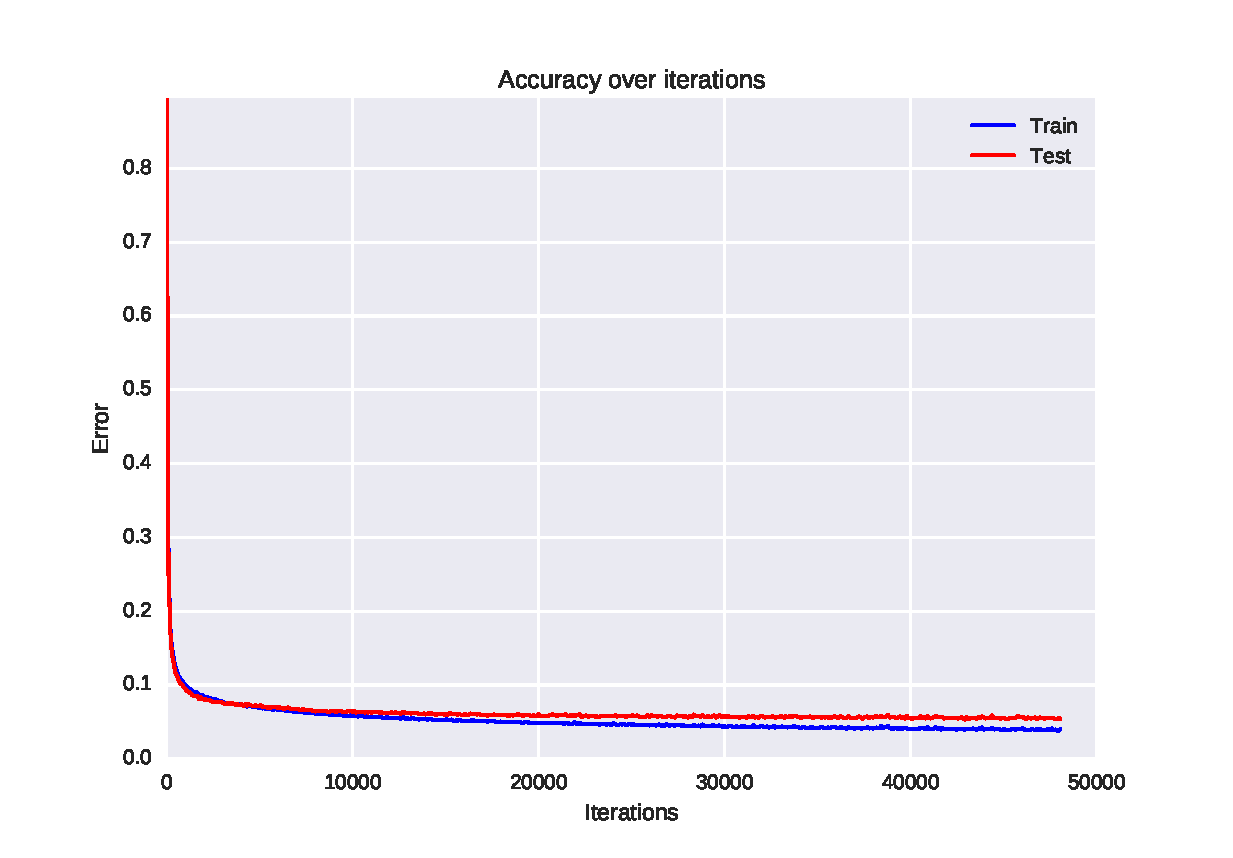
\includegraphics[width=0.95\textwidth]{error_model_2c.eps}
  \caption{Error plot for model 2c}
  \label{fig:err_2c}
\end{figure}

\begin{figure}[H]
  \centering
  \includegraphics[width=0.95\textwidth]{model_2c_confusion_matrix.eps}
  \caption{Confusion matrix for model 2c}
  \label{fig:conf_2c}
\end{figure}

Output of training and test error during training of the model. Due to the large
number of epochs we only show output of every ten epoch and the final epoch.

\verbatiminput{./code/Part2/model_2c_output.txt}

\begin{description}
\item[Final train error:] $0.03933$
\item[Final test error:] $0.05550$
\end{description}

\newpage

\subsection{Error table}

\begin{center}
  \begin{tabular}{ |c|c|c|c|c|c|c|c|c| } 
    \hline
    Experiment & P1:a & P1:b & P1:c & P1:d & P2:b & P2:c & P2:d & P2:e \\
    \hline
    Training error rate & 0.06973 & 0.00169 & 0.00000 & 0.00707 & 0.06604 & 0.04887 & 0.03933 & -\\ 
    Test error rate & 0.07620 & 0.02140 & 0.01890 & 0.01400 & 0.07300 & 0.06150 & 0.05550 & - \\ 
    \hline
  \end{tabular}
\end{center}

\end{document}
